\documentclass[10pt]{beamer}

\usetheme[progressbar=frametitle]{metropolis}
\usepackage{appendixnumberbeamer}

\usepackage{booktabs}
\usepackage[scale=2]{ccicons}

\usepackage{pgfplots}
\usepgfplotslibrary{dateplot}

\usepackage{xspace}
\newcommand{\themename}{\textbf{\textsc{metropolis}}\xspace}

\usepackage{tikz}
\usetikzlibrary{shapes,arrows}

\newcommand{\fcy}[1]{\mathcal{#1}}
\newcommand{\lit}[1]{\text{``#1''}}
\newcommand{\etag}[1]{\textsf{#1}}
\newcommand{\p}[2]{\langle #1, #2 \rangle}

\title{Typed Interactions for NLU in Opal}
\subtitle{Ongoing Research with Adrian Sampson}
% \date{\today}
\date{}
\author{Harrison Goldstein}
\institute{Cornell University}
% \titlegraphic{\hfill\includegraphics[height=1.5cm]{logo.pdf}}

\tikzstyle{block} = [rectangle, draw, fill=orange!20, text width=5em, text centered, minimum height=3em]
\tikzstyle{line} = [draw, -latex']
\tikzstyle{cloud} = [draw, ellipse,fill=red!20, node distance=3cm, minimum height=3em]

\begin{document}

\maketitle

\begin{frame}{Outline}
  \setbeamertemplate{section in toc}[sections numbered]
  \tableofcontents[hideallsubsections]
\end{frame}

\section{Motivation}

\begin{frame}[fragile]{An Example}

  We want to write a chat bot that will send messages between two users.

  ~\\
  It should be able to {\bf read} all messages that have been sent, and {\bf
    send} a message at a specified time (now or later).

  ~\\
  We want our bot to understand natural language.
\end{frame}

\begin{frame}[fragile]{Some Types}

  \begin{center}
    \begin{verbatim}
    type Msg = string;
    type Time = "now" | "later";
    type Send = {
      msg: Msg,
      time: Time
    };
    type Intent =
      | { kind: "Read", data: {} }
      | { kind: "Send", data: Send };
    \end{verbatim}
  \end{center}
\end{frame}

\begin{frame}[fragile]{Wit}

  Wit is a Natural Language Understanding tool developed with the help of
  Facebook.

  ~\\
  It has a relatively simple interface for training and interfacing with a NLU
  algorithm.

  ~\\
  Most of our work so far is tailored to Wit specifically, although we suspect
  that it could be translated to other NLU tools relatively easily.
\end{frame}

\begin{frame}[fragile]{The Goal}

  \begin{center}
    \begin{verbatim}
    "Tell Adrian to come to my talk, now."

    ==>

    {
      kind: "Send",
      data: {
        msg: "come to my talk",
        time: "now"
      }
    }
    \end{verbatim}
  \end{center}
\end{frame}

\begin{frame}[fragile]{The Goal}

  \begin{center}
    \begin{verbatim}
    "Read messages."

    ==>

    {
      kind: "Read",
      data: {}
    }
    \end{verbatim}
  \end{center}
\end{frame}

\begin{frame}[fragile]{Pitfalls}

  Unfortunately, NLU libraries, Wit included, tend to return a bag of entities
  with no real structure.

  ~\\
  There is no way to tell the library that entities depend on one-another (e.g.
  \verb|Send| contains a \verb|Msg|).

  ~\\
  Configuration and code are updated separately and could be inconsistent,
  resulting in broken applications.
\end{frame}

\section{Types for NLU}

\begin{frame}[fragile]{Finding Structure}

  Wit uses a three main ``search strategies'' to extract entities.

  ~\\
  \begin{columns}[T,onlytextwidth]
    \column{0.30\textwidth}
    {\bf Free Text}

    ~\\
    Captures a string of text. May have a certain form, or be found in a certain
    part of a sentence.

    ~\\
    E.g. message, address

    \column{0.30\textwidth}
    {\bf Keywords}

    ~\\
    Matches a specific word from a given set.

    ~\\~\\~\\~\\
    E.g. colors, months, now/later

    \column{0.30\textwidth}
    {\bf Trait}

    ~\\
    Slightly more abstract. Captures something that is defined by the utterance
    as a whole.

    ~\\
    E.g. mood, intent
  \end{columns}
\end{frame}

\begin{frame}[fragile]{Strategies as Types}

  If you squint hard enough, search strategies sort of look like types.

  ~\\
  One could imagine an NLU library using this fact to provide a safer
  interface---we haven't found any that do this.

  ~\\
  Our type language for NLU interactions captures these strategies in the types.
\end{frame}

\begin{frame}[fragile]{Type DSL}

  \begin{center}
    \begin{verbatim}
    free-text Msg;
    keywords Time = "now" | "later";
    type Send = {
      msg: Msg,
      time: Time
    };
    trait Intent = <Read> {} | <Send> Send;
    \end{verbatim}
  \end{center}
\end{frame}

\begin{frame}[fragile]{A Formal Specification}
  \begin{align*}
    \fcy{D} ::=&\ \text{FreeText}(\etag{t}) \\
    |&\ \text{KeyWords}(\etag{t},\ [\ell]) \\
    |&\ \text{Trait}(\etag{t},\ [\p{s}{\fcy{T}}]) \\
    |&\ \text{Type}(\etag{t},\ \fcy{T}) \\
    \\
    \fcy{T} ::=&\ \etag{t} \mid \ell \mid [\p{s}{\fcy{T}}] \mid \dots
  \end{align*}

  $$ t \in \textsc{Tag} \qquad \ell \in \textsc{Label} \qquad s \in
  \textbf{string} $$
\end{frame}

\section{Current Development}

\begin{frame}[fragile]{A First Attempt}

  \begin{center}
    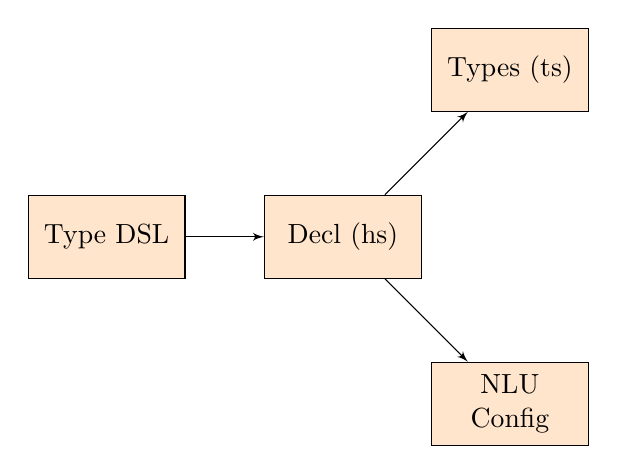
\begin{tikzpicture}[node distance = 3cm, auto]
      \node [block] (types) {Type DSL};
      \node [block, right of=types] (decls_hs) {Decl (hs)};
      \node [block, below right of=decls_hs] (cfg) {NLU Config};
      \node [block, above right of=decls_hs] (ts_types) {Types (ts)};

      \path [line] (types) -- (decls_hs);
      \path [line] (decls_hs) -- (cfg);
      \path [line] (decls_hs) -- (ts_types);
    \end{tikzpicture}
  \end{center}
\end{frame}

\begin{frame}[fragile]{Remember the Goal}

  \begin{center}
    \begin{verbatim}
    "Tell Adrian to come to my talk, now."

    ==>

    {
      kind: "Send",
      data: {
        msg: "come to my talk",
        time: "now"
      }
    }
    \end{verbatim}
  \end{center}
\end{frame}

\begin{frame}[fragile]{Wit's Response}

  \begin{center}
    \begin{verbatim}
    {
      Intent: [{
        value: "Send",
        confidence: 0.7
      }],
      Msg: [{
        value: "..."
        confidence: 0.9
      }],
      Time: [{
        value: "now",
        confidence: 0.6
      }]
    }
    \end{verbatim}
  \end{center}
\end{frame}

\begin{frame}[fragile]{Our Solution}

  \begin{center}
    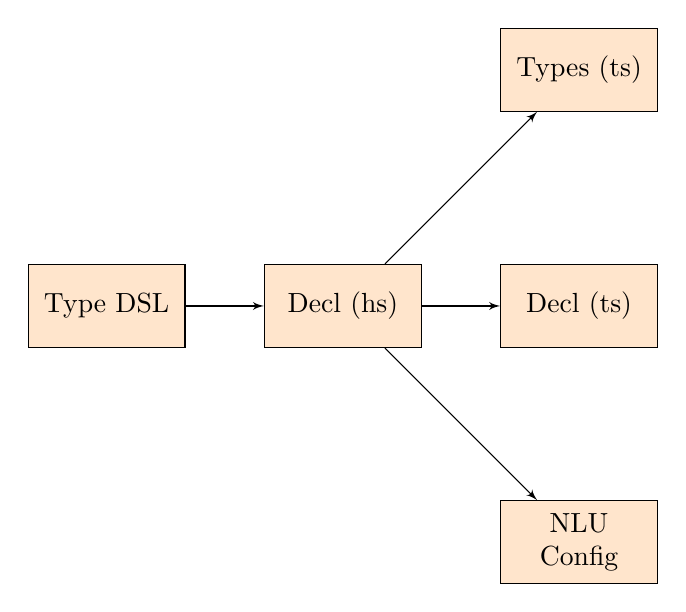
\begin{tikzpicture}[node distance = 3cm, auto]
      \node [block] (types) {Type DSL};
      \node [block, right of=types] (decls_hs) {Decl (hs)};
      \node [block, right of=decls_hs] (decls_ts) {Decl (ts)};
      \node [block, below of=decls_ts] (cfg) {NLU Config};
      \node [block, above of=decls_ts] (ts_types) {Types (ts)};

      \path [line] (types) -- (decls_hs);
      \path [line] (decls_hs) -- (decls_ts);
      \path [line] (decls_hs) -- (cfg);
      \path [line] (decls_hs) -- (ts_types);
    \end{tikzpicture}
  \end{center}
\end{frame}

\begin{frame}[fragile]{Parsing a Response}

  \begin{columns}
    \column{0.5\textwidth}
    \begin{center}
      \begin{verbatim}
      {
        Intent: [{
          value: "Send",
          confidence: 0.7
        }],
        Msg: [{
          value: "..."
          confidence: 0.9
        }],
        Time: [{
          value: "now",
          confidence: 0.6
        }]
      }
      \end{verbatim}
    \end{center}

    \column{0.5\textwidth}
    \begin{center}
      \begin{verbatim}
      {
        kind: ___,
        data: ___
      }
      \end{verbatim}
    \end{center}

  \end{columns}
\end{frame}

\begin{frame}[fragile]{Parsing a Response}

  \begin{columns}
    \column{0.5\textwidth}
    \begin{center}
      \begin{verbatim}
      {
        Intent: [{
          value: "Send",
          confidence: 0.7
        }],
        Msg: [{
          value: "..."
          confidence: 0.9
        }],
        Time: [{
          value: "now",
          confidence: 0.6
        }]
      }
      \end{verbatim}
    \end{center}

    \column{0.5\textwidth}
    \begin{center}
      \begin{verbatim}
      {
        kind: "Send",
        data: {
          msg: ___,
          time: ___
        }
      }
      \end{verbatim}
    \end{center}

  \end{columns}
\end{frame}

\begin{frame}[fragile]{Parsing a Response}

  \begin{columns}
    \column{0.5\textwidth}
    \begin{center}
      \begin{verbatim}
      {
        Intent: [{
          value: "Send",
          confidence: 0.7
        }],
        Msg: [{
          value: "..."
          confidence: 0.9
        }],
        Time: [{
          value: "now",
          confidence: 0.6
        }]
      }
      \end{verbatim}
    \end{center}

    \column{0.5\textwidth}
    \begin{center}
      \begin{verbatim}
      {
        kind: "Send",
        data: {
          msg: "...",
          time: "now"
        }
      }
      \end{verbatim}
    \end{center}

  \end{columns}
\end{frame}

\begin{frame}[fragile]{Our Solution}

  \begin{center}
    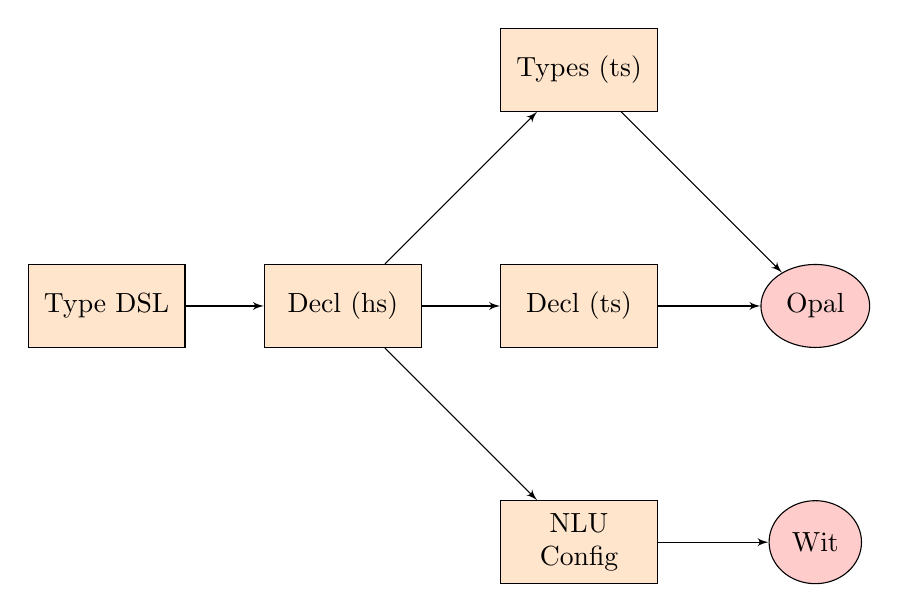
\begin{tikzpicture}[node distance = 3cm, auto]
      \node [block] (types) {Type DSL};
      \node [block, right of=types] (decls_hs) {Decl (hs)};
      \node [block, right of=decls_hs] (decls_ts) {Decl (ts)};
      \node [block, below of=decls_ts] (cfg) {NLU Config};
      \node [block, above of=decls_ts] (ts_types) {Types (ts)};
      \node [cloud, right of=decls_ts] (ts) {Opal};
      \node [cloud, right of=cfg] (backend) {Wit};

      \path [line] (types) -- (decls_hs);
      \path [line] (decls_hs) -- (decls_ts);
      \path [line] (decls_hs) -- (cfg);
      \path [line] (decls_hs) -- (ts_types);
      \path [line] (decls_ts) -- (ts);
      \path [line] (ts_types) -- (ts);
      \path [line] (cfg) -- (backend);
    \end{tikzpicture}
  \end{center}
\end{frame}

\section{Demo}
\section{Future Work}

\begin{frame}[fragile]{Future Work}

  \begin{itemize}
  \item More Types
    $$ \fcy{T} ::=\ \etag{t} \mid \ell \mid [\p{s}{\fcy{T}}] \mid \dots $$
  \item More Backends
    \begin{itemize}
    \item Support for more search strategies
    \item Generate multiple forms of configuration
    \end{itemize}
  \item Use Confidence Information
  \item Unit Tests as Training Samples
  \end{itemize}
\end{frame}

\end{document}